
If your application seems to run slow, then you might want to know where all the time is spent in the code. In this case, instrumenting the code with XRay helps you. Basically, at each function entry and exit, a special call into the runtime library is inserted. This allows counting how often a function is called, and also how much time is spent in the function. You find the implementation for the instrumentation pass in the llvm/lib/XRay/directory. The runtime portion is part of compiler-rt.\par

In the following example source, real work is simulated by calling the usleep() function. The func1() function sleeps for 10 μs. The func2() function either calls func1() or sleeps for 100 μs, depending on whether the n parameter is odd or even. Inside the main() function, both functions are called inside a loop. This is already enough to get interesting information. You'll need to save the following source code in the xraydemo.c file:\par

\begin{lstlisting}[caption={}]
#include <unistd.h>

void func1() { usleep(10); }

void func2(int n) {
	if (n % 2) func1();
	else usleep(100);
}

int main(int argc, char *argv[]) {
	for (int i = 0; i < 100; i++) { func1(); func2(i); }
	return 0;
}
\end{lstlisting}

To enable the XRay instrumentation during compilation, you will need to specify the -fxray-instrument option. Functions with less than 200 instructions are not instrumented. This is an arbitrary threshold defined by the developers, and in our case, the functions would not be instrumented. The threshold can be specified with the -fxrayinstruction-threshold= option. Alternatively, we can add a function attribute to control whether a function should be instrumented. For example, adding the following prototype would result in always instrumenting the function:\par

\begin{lstlisting}[caption={}]
void func1() __attribute__((xray_always_instrument));
\end{lstlisting}

Likewise, by using the xray\underline{~}never\underline{~}instrument attribute, you can turn off
instrumentation for a function.\par

We will now use the command-line option and compile the xraydemo.c file as follows:\par

\begin{tcolorbox}[colback=white,colframe=black]
\$ clang -fxray-instrument -fxray-instruction-threshold=1 -g $\setminus$ \\
\hspace*{1cm}xraydemo.c -o xraydemo
\end{tcolorbox}

In the resulting binary, instrumentation is turned off by default. If you run the binary, you will note no difference to a not-instrumented binary. The XRA\underline{~}OPTIONS environment variable is used to control the recording of runtime data. To enable data collection, you run the application as follows:\par

\begin{tcolorbox}[colback=white,colframe=black]
\$ XRAY\underline{~}OPTIONS= "patch\underline{~}premain=true xray\underline{~}mode=xray-basic "$\setminus$ \\
./xraydemo
\end{tcolorbox}

The xray\underline{~}mode=xray-basic option tells the runtime that we want to use basic mode. In this mode, all runtime data is collected, which can result in huge log files. When the patch\underline{~}premain=true option is given, then functions that are run before the main() function are instrumented, too.\par

After running this command, you see a new file in the directory, in which the collected data is stored. You need to use the llvm-xray tool to extract readable information from this file.\par

The llvm-xray tool supports various subcommands. You use the account
subcommand to extract some basic statistics. For example, to get the top 10 most called functions, you add the -top=10 option to limit the output, and the -sort=count option to specify the function call count as the sort criteria. You can influence the sort order with the -sortorder= option. Run the following command to get the statistic:\par

\begin{tcolorbox}[colback=white,colframe=black]
\$ llvm-xray account xray-log.xraydemo.xVsWiE -sort=count$\setminus$ \\
\hspace*{0.5cm}-sortorder=dsc -instr\underline{~}map ./xraydemo \\
Functions with latencies: 3 \\
\hspace*{0.5cm}funcid \hspace{1cm}count \hspace{2cm}sum \hspace{1cm}function \\
\hspace*{1.4cm}1\hspace{1.4cm}150\hspace{1.4cm}0.166002 \hspace{1cm}demo.c:4:0: func1 \\
\hspace*{1.4cm}2\hspace{1.4cm}100\hspace{1.4cm}0.543103 \hspace{1cm}demo.c:9:0: func2 \\
\hspace*{1.4cm}3\hspace{1.8cm}1 \hspace{1.3cm}0.655643 \hspace{1cm}demo.c:17:0: main
\end{tcolorbox}

You can see that the func1() function is called most often, as well as the accumulated time spent in this function. The example only has three functions, so the –top= option has no visible effect here, but for real applications, it is very useful.\par

From the collected data, it is possible to reconstruct all the stack frames that occurred during runtime. You use the stack subcommand to view the top 10 stacks. The output shown here is reduced for brevity:\par

\begin{tcolorbox}[colback=white,colframe=black]
\$ llvm-xray stack xray-log.xraydemo.xVsWiE -instr\underline{~}map$\setminus$ \\
\hspace*{0.5cm}./xraydemo \\
Unique Stacks: 3 \\
Top 10 Stacks by leaf sum:\\
\\
Sum: 1325516912\\
lvl \hspace{1cm}function \hspace{2.5cm}count \hspace{2.5cm}sum\\
\#0\hspace{1.5cm}main \hspace{3.3cm}1 \hspace{1.3cm}1777862705 \\
\#1\hspace{1.5cm}func2 \hspace{3.0cm}50 \hspace{1.35cm}1325516912 \\
\\
Top 10 Stacks by leaf count:\\
\\
Count: 100 \\
lvl \hspace{1cm}function \hspace{2.5cm}count \hspace{2.5cm}sum \\
\#0\hspace{1.5cm}main \hspace{3.3cm}1 \hspace{1.3cm}1777862705 \\
\#1\hspace{1.5cm}func1 \hspace{2.9cm}100 \hspace{1.45cm}303596276
\end{tcolorbox}

A stack frame is a sequence of how a function is called. The func2() function is called by the main() function, and this is the stack frame with the largest accumulated time. The depth depends on how many functions are called, and the stack frames are usually large.\par

This subcommand can also be used to create a flame graph from the stack frames. With a flame graph, you can easily identify which functions have a large accumulated runtime. The output is the stack frames with count and runtime information. Using the flamegraph.pl script, you convert the data into a Scalable Vector Graphics (SVG) file, which you can view in your browser.\par

With the following command, you instruct llvm-xray to output all stack frames with the –all-stacks option. Using the –stack-format=flame option, the output is in the format expected by the flamegraph.pl script. With the –aggregationtype option, you can choose whether stack frames are aggregated by total time or by the number of invocations. The output of llvm-xray is piped into the flamegraph.pl script, and the resulting output is saved in the flame.svg file:\par

\begin{tcolorbox}[colback=white,colframe=black]
\$ llvm-xray stack xray-log.xraydemo.xVsWiE -all-stacks$\setminus$ \\
\hspace*{0.5cm}-stack-format=flame \verb|--|aggregation-type=time$\setminus$ \\
\hspace*{0.5cm}-instr\underline{~}map ./xraydemo | flamegraph.pl >flame.svg
\end{tcolorbox}

Open the generated flame.svg file in your browser. The graphic looks as follows:\par

\hspace*{\fill} \par %插入空行
\begin{center}
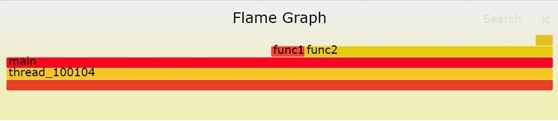
\includegraphics[width=1\textwidth]{content/3/chapter11/images/1.jpg}\\
Figure 11.1 – Flame graph produced by llvm-xray
\end{center}

Flame graphs can be confusing at the first look, because the x axis does not have the usual meaning of elapsed time. Instead, the functions are simply sorted by name. The colors are chosen to have good contrast and have no other meaning. From the preceding graph, you can easily determine the call hierarchy and the time spent in a function.\par

Information about a stack frame is displayed only after you move the mouse cursor over the rectangle representing the frame. With a mouse click on the frame, you can zoom into this stack frame. Flame graphs are of great help i f you want to identify functions worth optimizing. To find out more about flame graphs, please visit the website of Brendan Gregg, the inventor of flame graphs, \url{http://www.brendangregg.com/
flamegraphs.html}.\par

You can use the convert subcommand to convert the data into .yaml format or into the format used by the Chrome trace viewer visualization. The latter is another nice way to create a graphic from the data. To save the data in the xray.evt file, you run the following command:\par

\begin{tcolorbox}[colback=white,colframe=black]
\$ llvm-xray convert -output-format=trace\underline{~}event$\setminus$ \\
\hspace*{0.5cm}-output=xray.evt -symbolize –sort$\setminus$ \\
\hspace*{0.5cm}-instr\underline{~}map=./xraydemo xray-log.xraydemo.xVsWiE
\end{tcolorbox}

If you do not specify the –symbolize option, then no function names are shown in the resulting graph.\par

Once that is done, open the Chrome browser and type chrome:///tracing. Then, click on the Load button to load the xray.evt file. You will see the following visualization of the data:\par

\hspace*{\fill} \par %插入空行
\begin{center}
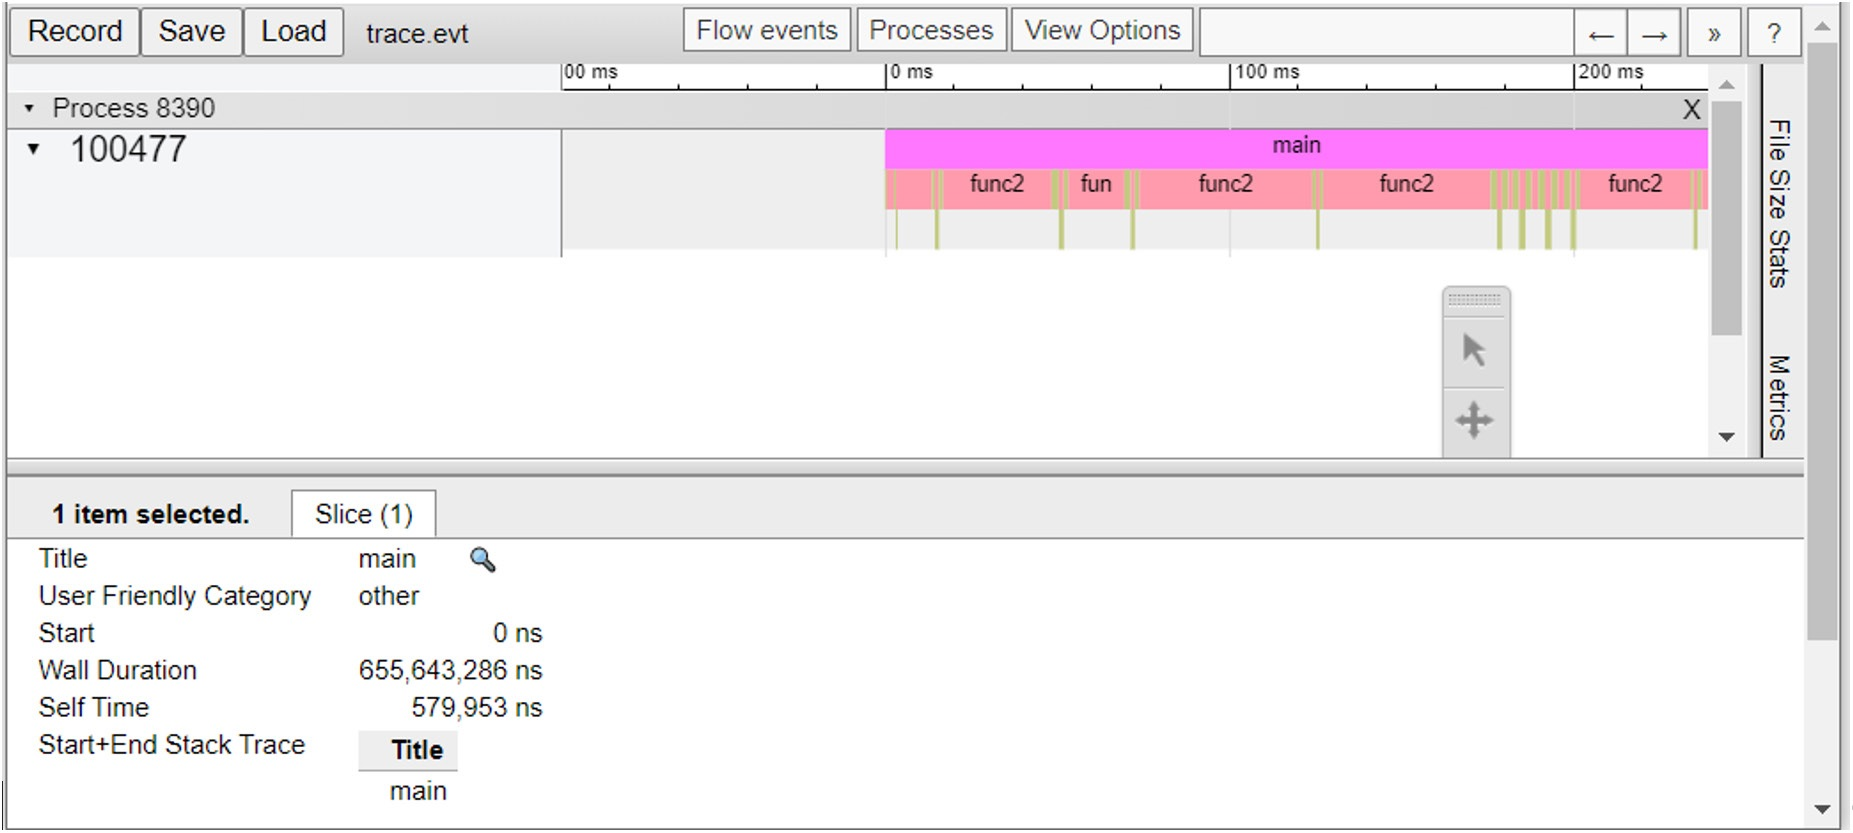
\includegraphics[width=1\textwidth]{content/3/chapter11/images/2.jpg}\\
Figure 11.2 – Chrome trace viewer visualization generated by llvm-xray
\end{center}

In this view, the stack frames are sorted by the time the function call occurs. For further interpretation of the visualization, please read the tutorial at \url{https://www.chromium.org/developers/how-tos/trace-event-profiling-tool}.

\begin{tcolorbox}[colback=blue!5!white,colframe=blue!75!black, title=Tip]
The llvm-xray tool has more functionality. You can read about it on the LLVM website at \url{https://llvm.org/docs/XRay.html} and \url{https://llvm.org/docs/XRayExample.html}.
\end{tcolorbox}

In this section, we learned how to instrument an application with XRay, how to collect runtime information, and how to visualize that data. We can use this knowledge to find performance bottlenecks in applications.\par

Another approach to identifying errors in an application is to analyze the source code, which is done with the static analyzer.\par
















